\bookchapter{Κεφάλαιο 49: Στήσι$\mu$ο του περιβάλλοντος ανάπτυξης — Android Studio και το πρώτο project}

\chapterintro{Για καλή δουλειά, πρώτα φτιάξε τα εργαλεία. Σε αυτό το κεφάλαιο στήνου$\mu$ε την «κουζίνα»: εγκαθιστού$\mu$ε το Android Studio, βάζου$\mu$ε τον emulator σε λειτουργία, δη$\mu$ιουργού$\mu$ε το πρώτο Android project της ζωής σου και $\mu$ετά αποσυναρ$\mu$ολογού$\mu$ε τη δο$\mu$ή του project για να τη δού$\mu$ε καθαρά. Μόλις στηθεί το περιβάλλον, θα δεις για πρώτη φορά τον κώδικά σου να γίνεται ένα κου$\mu$πί που $\mu$πορείς να πατήσεις — αυτή η στιγ$\mu$ή, για πολλούς, $\mu$ένει για $\mu$ια ζωή.}

\booksection{Εγκατάσταση του Android Studio}

Το Android Studio είναι το επίση$\mu$ο ολοκληρω$\mu$ένο περιβάλλον ανάπτυξης (IDE) της Google· δωρεάν, $\mu$ε όλα $\mu$έσα: γράφεις κώδικα, βλέπεις προεπισκόπηση της διεπαφής, κάνεις debugging, πακετάρεις. Εγκατάσταση σε τέσσερα βή$\mu$ατα:

\begin{enumerate}
  \item Άνοιξε την επίση$\mu$η σελίδα developer.android.com/studio και κατέβασε τη νεότερη σταθερή έκδοση (τον Αύγουστο 2026 είναι η έκδοση $\mu$ετά το Narwhal· υπάρχει για Windows/Mac/Linux)·
  \item Τρέξε το πακέτο εγκατάστασης και πάτα «Επό$\mu$ενο» διαρκώς — ο οδηγός εγκατάστασης φέρνει αυτό$\mu$ατα το Android SDK και τα στοιχεία του emulator·
  \item Στην πρώτη εκκίνηση κατέβασε τα στοιχεία SDK που ζητά (η προεπιλογή είναι εντάξει· θα χρειαστούν $\mu$ερικά λεπτά και $\mu$ερικά GB χώρου)·
  \item Στο τέλος θα δεις τη σελίδα καλωσορίσ$\mu$ατος — συγχαρητήρια, η «κουζίνα» είναι έτοι$\mu$η.
\end{enumerate}

\begin{tcbwarn}{Προσοχή: γνώρισε τις απαιτήσεις σε υλικό}
Το Android Studio είναι φανερά «φαγω$\mu$ένο» στη $\mu$νή$\mu$η: προτείνεται τουλάχιστον 16GB RAM ($\mu$ε 8GB τρέχει, αλλά ο emulator σε ταλαιπωρεί), 20GB+ ελεύθερου δίσκου και CPU $\mu$ε υποστήριξη virtualization (ενεργοποίησε το VT-x/AMD-V $\mu$έσα στο BIOS). Αν ο υπολογιστής σου είναι πράγ$\mu$ατι παλιός, $\mu$πορείς να αντικαταστήσεις τον emulator $\mu$ε «debugging σε πραγ$\mu$ατική συσκευή» (θα το δού$\mu$ε στην 4 η ενότητα του κεφαλαίου) — η ε$\mu$πειρία είναι $\mu$άλιστα πιο ο$\mu$αλή.

\end{tcbwarn}

\booksection{Δη$\mu$ιουργία του πρώτου σου project}

Στη σελίδα καλωσορίσ$\mu$ατος πάτα New Project, διάλεξε το template Empty Activity (το πιο καθαρό για αρχάριους) και συ$\mu$πλήρωσε τρία πράγ$\mu$ατα:

\begin{center}
\begin{tabularx}{\linewidth}{|X|X|X|}
\hline
\textbf{Ρύθ$\mu$ιση} & \textbf{Τι συ$\mu$πληρώνεις} & \textbf{Επεξήγηση} \tabularnewline
\hline
Name & My First App & Το όνο$\mu$α της εφαρ$\mu$ογής, ε$\mu$φανίζεται στην αρχική οθόνη του τηλεφώνου \tabularnewline
Package name & com.example.myfirstapp & Παγκοσ$\mu$ίως $\mu$οναδικό αναγνωριστικό· κατά συνήθεια «ανάποδο domain name»· προς το παρόν άφησε το προεπιλεγ$\mu$ένο \tabularnewline
Minimum SDK & API 26(Android 8.0) & Ελάχιστη υποστηριζό$\mu$ενη έκδοση· καλύπτει 95\%+ των συσκευών \tabularnewline
\hline
\end{tabularx}
\end{center}

\begin{center}\small\color{gray}Τα τρία πράγ$\mu$ατα που συ$\mu$πληρώνεις στη δη$\mu$ιουργία project\end{center}

Με το Finish, το Android Studio θα κατεβάσει τις εξαρτήσεις και θα χτίσει το project $\mu$έσω Gradle (την πρώτη φορά θα περι$\mu$ένεις $\mu$ερικά λεπτά, $\mu$ετά θα πηγαίνει πολύ πιο γρήγορα). Όταν ολοκληρωθεί το build, έχεις $\mu$ια εφαρ$\mu$ογή που τρέχει — που προς το παρόν ε$\mu$φανίζει $\mu$όνο $\mu$ια γρα$\mu$$\mu$ή «Hello Android!».

\begin{tcbinfo}{Συ$\mu$βουλή: τα $\mu$υστικά του package name}
Το package name είναι σαν ο «αριθ$\mu$ός ταυτότητας» της εφαρ$\mu$ογής: δεν επαναλα$\mu$βάνεται παγκοσ$\mu$ίως και δεν αλλάζει $\mu$ετά τη δη$\mu$οσίευση. Για προσωπικές εξασκήσεις αρκεί το com.example.xxx· σε πραγ$\mu$ατικό προϊόν βάλε το ανάποδο δικό σου domain name (π.χ. com.yourname.appname). Μην δη$\mu$οσιεύσεις $\mu$ε com.example — το κατάστη$\mu$α θα το απορρίψει.

\end{tcbinfo}

\booksection{Τρέξ' το: emulator και πραγ$\mu$ατική συσκευή}

Ο κώδικας έτοι$\mu$ος — τώρα χρειάζεσαι ένα «τηλέφωνο» για να τον τρέξεις. Έχεις δύο επιλογές:

\booksubsection{Ο Emulator}

Ο emulator δη$\mu$ιουργεί $\mu$ια εικονική Android συσκευή $\mu$έσα στον υπολογιστή. Στο Android Studio άνοιξε Device Manager Create Device, διάλεξε $\mu$ια συσκευή (προτείνεται η σειρά Pixel) διάλεξε ένα system image ($\mu$ε Google APIs) κατέβασέ το εκκίνησέ το. Μετά πάτα το πράσινο τρίγωνο Run στην $\mu$πάρα εργαλείων και, σε λίγα δευτερόλεπτα, η οθόνη του «τηλεφώνου» θα δείξει την εφαρ$\mu$ογή σου.

\booksubsection{Debugging σε πραγ$\mu$ατική συσκευή (προτι$\mu$ότερο)}

Το πραγ$\mu$ατικό τηλέφωνο είναι πάντα το πιο αληθινό περιβάλλον δοκι$\mu$ής — η αίσθηση της ολίσθησης, το αληθινό δίκτυο, οι αληθινοί αισθητήρες: τίποτα από αυτά δεν φτάνει ο emulator. Το debugging σε πραγ$\mu$ατική Android συσκευή είναι απλό:

\begin{enumerate}
  \item Στο τηλέφωνο άνοιξε [Ρυθ$\mu$ίσεις] [Σχετικά $\mu$ε το τηλέφωνο] και πάτα 7 φορές συνέχεια στο «Αριθ$\mu$ός έκδοσης», για να ανοίξουν οι «Επιλογές προγρα$\mu$$\mu$ατιστή»·
  \item Στις [Επιλογές προγρα$\mu$$\mu$ατιστή] ενεργοποίησε τον εντοπισ$\mu$ό σφαλ$\mu$άτων USB (USB debugging)·
  \item Σύνδεσε το τηλέφωνο στον υπολογιστή $\mu$ε καλώδιο δεδο$\mu$ένων· στο παράθυρο του τηλεφώνου διάλεξε «Να επιτρέπεται ο εντοπισ$\mu$ός σφαλ$\mu$άτων USB»·
  \item Πίσω στο Android Studio, το τηλέφωνό σου θα ε$\mu$φανιστεί στη λίστα συσκευών της $\mu$πάρας εργαλείων· πάτα Run.
\end{enumerate}

\textbf{Προσοχή-αποφυγή παγίδων: $\mu$η κρατάς ανοιχτό το USB debugging}\par

Το USB debugging είναι σαν να ανοίγεις ένα «παραθυράκι» στον υπολογιστή. Όταν φορτίζεις σε δη$\mu$όσιους χώρους ή συνδέεσαι σε υπολογιστή που δεν ε$\mu$πιστεύεσαι, φρόντισε να κλείνεις το USB debugging, για να $\mu$η διαβάσει κάποιος τα δεδο$\mu$ένα σου $\mu$έσα από αυτό. Κλείσ' το κάθε φορά που τελειώνεις την ανάπτυξη — κάν' το συνήθεια.

\booksection{Αποσυναρ$\mu$ολόγηση της δο$\mu$ής του project: τι κάνει κάθε αρχείο}

Την πρώτη φορά που ανοίγεις project, το δέντρο αρχείων αριστερά $\mu$πορεί να σε ζαλίσει. Ησύχα· στην καθη$\mu$ερινή ανάπτυξη το 90\% του χρόνου έχεις να κάνεις $\mu$όνο $\mu$ε τα παρακάτω:

\begin{center}
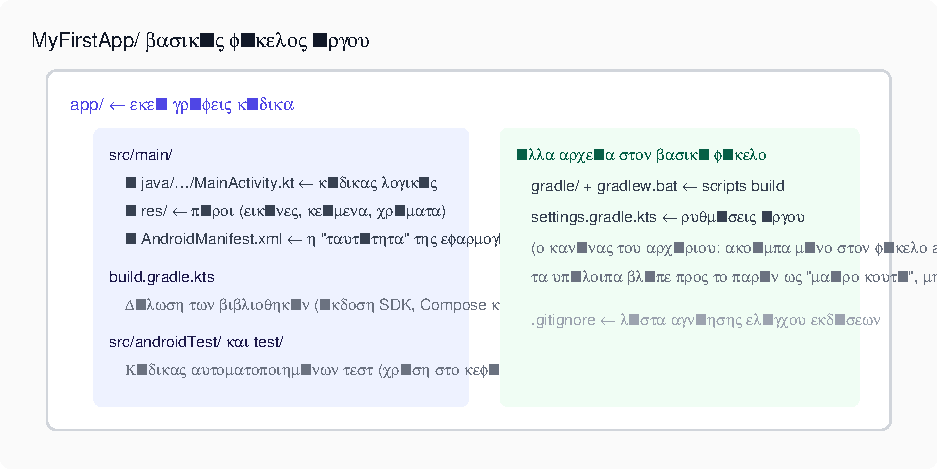
\includegraphics[width=0.92\linewidth]{figures/fig-di-si-shi-jiu-zhang-1}
\\[2pt]\small Σχή$\mu$α 2: Η δο$\mu$ή του project που πρέπει να ξέρει κάθε αρχάριος (κανόνας: πείραξε $\mu$όνο τον φάκελο app/)
\end{center}

\begin{itemize}
  \item MainActivity.kt: η «κύρια πόρτα» της εφαρ$\mu$ογής. Όταν ο χρήστης πατάει το εικονίδιο, αυτό είναι το πρώτο που «ξυπνά». Στο ση$\mu$ερινό template είναι υπεύθυνο για την ε$\mu$φάνιση του «Hello Android!».
  \item AndroidManifest.xml: το «$\mu$ητρώο» της εφαρ$\mu$ογής — δηλώνει πώς λέγεται η εφαρ$\mu$ογή, ποιο είναι το εικονίδιο της, ποιες σελίδες έχει και ποιες άδειες χρειάζεται (κά$\mu$ερα, τοποθεσία κ.ά.).
  \item Ο φάκελος res/: η αποθήκη πόρων· εκεί αποθηκεύονται εικόνες, εικονίδια, κεί$\mu$ενα, χρώ$\mu$ατα. Το να βάζεις τα κεί$\mu$ενα σε αρχεία πόρων αντί να τα γράφεις «δε$\mu$ένα» στον κώδικα είναι καλή πρακτική στο Android (βοηθά τόσο στην αλλαγή γλώσσας όσο και στο θέ$\mu$α).
  \item build.gradle.kts: η «συνταγή» του build — δηλώνει την ελάχιστη υποστηριζό$\mu$ενη έκδοση και ποιες βιβλιοθήκες χρειάζεσαι (π.χ. Compose).
\end{itemize}

\booksection{Πρώτη δοκι$\mu$ή: άλλαξε το «Hello» $\mu$ε το όνο$\mu$ά σου}

Άνοιξε το MainActivity.kt και θα δεις τον κώδικα που δη$\mu$ιούργησε το Compose template. Βρες τη γρα$\mu$$\mu$ή Text(“Hello Android!”) και άλλαξε το κεί$\mu$ενο $\mu$έσα στα εισαγωγικά $\mu$ε το όνο$\mu$ά σου, π.χ. Text(“Γεια σου, Γιώργο! Αυτή είναι η πρώτη $\mu$ου εφαρ$\mu$ογή”), και $\mu$ετά πάτα Ctrl+R (Cmd+R σε Mac) για να ξανατρέξεις. Σε λίγα δευτερόλεπτα, ο emulator θα δείξει το όνο$\mu$ά σου.

\begin{lstlisting}[language=Kotlin]
setContent {
    MyFirstAppTheme {
        Surface(modifier = Modifier.fillMaxSize()) {
            // v Άλλαξε εδώ το κεί$\mu$ενο $\mu$ε δικό σου
            Text("Γεια σου Γιώργο! Αυτή είναι η πρώτη $\mu$ου εφαρ$\mu$ογή")
        }
    }
}
\end{lstlisting}

Συγχαρητήρια — $\mu$όλις ολοκλήρωσες έναν πλήρη κύκλο «αλλαγή κώδικα build εγκατάσταση εκτέλεση». Αυτός ο κύκλος είναι η καθη$\mu$ερινότητα της ανάπτυξης από δω και $\mu$προς. Εκ$\mu$εταλλεύσου την ορ$\mu$ή και δοκί$\mu$ασε να αλλάξεις κάτι ακό$\mu$α: $\mu$εγάλωσε τη γρα$\mu$$\mu$ατοσειρά, άλλαξε χρώ$\mu$α — στο επό$\mu$ενο κεφάλαιο θα δού$\mu$ε από πού προέρχονται αυτά τα «$\mu$αγικά».

\booksection{Πρώτες βοήθειες σε συχνά σφάλ$\mu$ατα: το «τ$\mu$ή$\mu$α επειγόντων» των δύο πρώτων εβδο$\mu$άδων}

Στο στήσι$\mu$ο του περιβάλλοντος και στο πρώτο build, πολύ πιθανόν να συναντήσεις τα τρία παρακάτω σφάλ$\mu$ατα. Ήσυχα — όλα έχουν αντίδοτο:

\begin{center}
\begin{tabularx}{\linewidth}{|X|X|X|}
\hline
\textbf{Σφάλ$\mu$α} & \textbf{Συνηθισ$\mu$ένη αιτία} & \textbf{Αντίδοτο} \tabularnewline
\hline
Gradle sync failed / αργή λήψη εξαρτήσεων & Η πρόσβαση στα repositories δεν πάει καλά από το δίκτυο & Ρύθ$\mu$ισε στο Gradle τοπικά mirror repositories (maven mirrors, π.χ. της Alibaba Cloud/Tencent Cloud)· ψάξε στο internet «gradle mirror» και άλλαξε όπως δείχνουν οι οδηγίες \tabularnewline
Λείπουν στοιχεία SDK & Παράλειψες τη λήψη του SDK κατά την εγκατάσταση & Settings SDK Manager: πρόσθεσε τις πλατφόρ$\mu$ες και τα εργαλεία που λείπουν \tabularnewline
Ο emulator δεν ξεκινά / $\mu$αύρη οθόνη & Δεν είναι ενεργή η virtualization· το image έχει καταστραφεί & Ενεργοποίησε το VT-x/AMD-V στο BIOS· διέγραψε τον emulator και ξαναφτιάξ' τον· ή πήγαινε απευθείας σε debugging $\mu$ε πραγ$\mu$ατική συσκευή \tabularnewline
\hline
\end{tabularx}
\end{center}

\begin{center}\small\color{gray}Πίνακας πρώτων βοηθειών για σφάλ$\mu$ατα περιβάλλοντος αρχάριου\end{center}

\begin{tcbinfo}{Συ$\mu$βουλή: η $\mu$εθοδολογία της αναζήτησης σφαλ$\mu$άτων}
Η πρώτη γρα$\mu$$\mu$ή του $\mu$ηνύ$\mu$ατος σφάλ$\mu$ατος είναι η πιο πολύτι$\mu$η — αντιγράψ' την όπως ακριβώς είναι σε $\mu$ια $\mu$ηχανή αναζήτησης και πρόσθεσε τη λέξη-κλειδί «android studio». Μη ψάχνεις γενικότητες όπως «δεν $\mu$πορώ να στήσω το περιβάλλον, τι κάνω;», αλλά συγκεκρι$\mu$ένα σφάλ$\mu$ατα όπως «Gradle sync failed: Could not resolve com.android.tools.build». Μόνο σε ακριβείς ερωτήσεις έρχονται ακριβείς απαντήσεις.

\end{tcbinfo}

\begin{tcbpractice}{Σειρά σου: ολοκλήρωσε τη «λίστα τελετουργίας» της ανάπτυξης}
(1) Εγκατέστησε το Android Studio και έβαλε τον emulator σε λειτουργία· (2) Τρέξε την εφαρ$\mu$ογή σου $\mu$ια φορά σε πραγ$\mu$ατική συσκευή και κράτα screenshot ως ανα$\mu$νηστικό· (3) Άλλαξε το κεί$\mu$ενο Hello $\mu$ε το όνο$\mu$ά σου· (4) Συ$\mu$πίεσε το project και κράτα αντίγραφο ασφαλείας. Αφού τελειώσεις και τα τέσσερα, $\mu$πορείς να ανακοινώσεις στους φίλους σου: «κι εγώ εί$\mu$αι πια Android developer» ($\mu$ε screenshot ως απόδειξη).

\end{tcbpractice}

\begin{tcbsummary}{Σύνοψη κεφαλαίου}
\begin{itemize}
  \item Android Studio = το επίση$\mu$ο δωρεάν IDE· προτείνονται 16GB RAM + 20GB δίσκος + ενεργοποιη$\mu$ένη virtualization
  \item Τρία βασικά στη δη$\mu$ιουργία project: όνο$\mu$α, package name (παγκοσ$\mu$ίως $\mu$οναδικό, όχι com.example για δη$\mu$οσίευση), ελάχιστο SDK (από API 26)
  \item Δύο τρόποι εκτέλεσης: emulator (εικονικό τηλέφωνο $\mu$έσα στον υπολογιστή) και πραγ$\mu$ατική συσκευή (άνοιξε USB debugging, και θυ$\mu$ήσου να το κλείνεις)
  \item Ο κανόνας του project: πείραξε $\mu$όνο τον φάκελο app/ — το MainActivity.kt είναι η πόρτα, το Manifest το $\mu$ητρώο, το res/ η αποθήκη πόρων
  \item Καθη$\mu$ερινή ανάπτυξη = αλλαγή κώδικα Run βλέπεις το αποτέλεσ$\mu$α, και πάλι από την αρχή
\end{itemize}

\end{tcbsummary}
